\documentclass[11pt,letterpaper]{article}
\usepackage{graphicx}
\usepackage{geometry}
\usepackage{amsmath}
\usepackage{hyperref}
\usepackage{url}
\usepackage{natbib}
\usepackage{booktabs}
\usepackage{xcolor}
\usepackage{listings}
\geometry{margin=1in}
\hypersetup{colorlinks=true, linkcolor=black, citecolor=black, urlcolor=black}

\title{When Repair Levers Combine, Machine Translation Editing Gets Worse}
\author{}
\date{}

\begin{document}
\maketitle

\begin{abstract}
Automatic quality-estimation (QE) systems can flag likely translation errors without a human reference, raising the possibility of scoped editing: repairing only the flagged span instead of retranslating the whole sentence. The one shared-task test of this idea placed a naive scoped-editing system dead last among eight ranked systems. We separate that design into two independently switchable levers -- localization breadth (how much of the sentence a checker may flag) and iteration (whether a repair is re-checked and re-repaired) -- and execute the full resulting factorial design plus a hygiene-only control, on a fixed repair model, a deterministic content-invariant checker, and the same real quality-estimation checkpoint for every condition. Broadening localization alone substantially narrows the quality gap relative to a faithful reproduction of the shared-task baseline, but at a real correctness cost: the checker's own target error is fixed far less reliably, and previously correct parts of the sentence get broken more often. Iterating alone, while keeping localization narrow, recovers nearly all of that correctness cost without improving whole-sentence quality. Combining both levers does not combine their gains. This iteration obtains the combined condition's quality score on the same real checkpoint used everywhere else in the study, after a checkpoint-access failure had forced a non-comparable substitute previously, and finds it statistically indistinguishable from the unedited baseline: the quality benefit of broadened localization does not survive being paired with iteration. On correctness, the combined condition's true regression rate is the highest of every condition tested, and the fraction of sentences reaching a fully verified state within a shared pass budget collapses once the checker's surface broadens to whole-sentence scope. A precision-stratified re-analysis shows this collapse concentrates in the checker categories where detection precision is lowest, consistent with -- though not proof of -- checker noise compounding the failure rather than damage spread uniformly across every checked invariant. The result disconfirms the hypothesis that broadened localization and iteration are complementary levers whose combination captures both gains: on every axis now measured with a shared, real metric, combining them produces the worst outcome of any condition tested.
\end{abstract}

\section{Introduction}

Machine translation systems increasingly ship with an automatic quality-estimation (QE) step that flags likely errors in a translation without needing a human reference \citep{Lavie2025}. The natural next question is whether those flags can drive automatic repair: instead of retranslating a whole sentence to fix one wrong number or dropped negation, an editing system could touch only the flagged span and leave the rest of the sentence -- which the base translator already got right -- untouched. This is \emph{scoped editing}: localize a problem with QE, then repair only that region. Scoped editing matters because a system that regenerates an entire sentence can silently break a correct number, name, or negation while fixing something else, and the total-sentence quality metrics used to score MT systems do not distinguish ``improved and stayed faithful'' from ``improved by chance while corrupting a different part of the sentence'' \citep{Rei2022}. In a regulated, terminology-heavy domain -- legal, medical, financial translation -- a single flipped number or negation is a severe, auditable failure independent of whether the sentence's aggregate quality score went up.

The 2025 WMT shared task on automated translation evaluation (Task 3, minimal editing) gave scoped editing its first head-to-head test against full retranslation \citep{Lavie2025}. A scoped-editing system that masks each QE-flagged span with a placeholder token and fills it with one pass of a small language model finished dead last among eight ranked systems, at $-0.0108$ mean $\Delta$COMET, while a second, independently built scoped-editing system in the same ranking landed near break-even \citep{Lavie2025,Padmanabhan2025}. Four iterations of this project separated the design space of that losing system into two independently switchable factors -- \emph{localization breadth} (how much of the sentence a checker is allowed to flag) and \emph{iteration} (whether a flagged repair is re-checked and re-repaired) -- and executed all five resulting conditions: broadening localization alone in a single uncorrected pass (Condition C1) cut the reproduced quality loss roughly fivefold in $\Delta$COMET terms, at a real cost, with fix rate on injected errors falling from 0.98 to 0.61 and true regression rate rising from 0.07 to 0.14 relative to narrow-localization baselines; iterating alone, holding localization narrow (Condition C2), recovered that fix-rate and regression-rate cost almost completely, but did not itself move $\Delta$COMET; and Condition C -- both levers combined -- was executed for the first time in the immediately prior iteration, disconfirming a ``best of both'' outcome on the two correctness axes fully measured, but leaving its quality axis unresolved: the real \texttt{wmt22-cometkiwi-da} checkpoint that scored every other condition in this protocol could not be downloaded during that run (HTTP 429 on twelve retry attempts across two backoff probes), forcing a substitute proxy metric with no established comparability to the other four conditions' real-COMET numbers.

This iteration closes that remaining gap and, in doing so, sharpens the paper's central finding into a decisive rather than a partial disconfirmation. A scoring-only rerun -- no new repair generation, no new repair-model calls -- obtained the real \texttt{wmt22-cometkiwi-da} checkpoint on its very first attempt this time, and Condition C's $\Delta$COMET is now directly comparable, on the identical metric, to every other condition in the study. It is $-0.0173$ (95\% CI $[-0.0251,-0.0103]$), statistically indistinguishable from the unedited faithful baseline's $-0.0164$ and from iteration-alone's $-0.0166$, and far worse than broadened-localization-alone's $-0.0035$. Combining the two levers does not just fail to combine their correctness gains, as the prior iteration showed; it also fails to combine their quality gains, now measured on the same footing as everything else in the study. A reviewer of the prior draft raised three further concerns this iteration addresses directly: whether the certificate-rate collapse behind Condition C's elevated regression rate is genuine cross-invariant damage or a confound with the checker's own imperfect precision; whether the paper's ``every condition can attempt'' comparison population silently mixed cells the checker can and cannot actually localize and verify; and whether a literature-search artifact's own flagged open item -- an unfetched EAMT 2026 paper -- was resolved before the novelty claim was finalized. All three are now closed with new evidence rather than argued away, detailed in Sections 6.6--6.8 and reflected throughout the Discussion.

\textbf{Summary of contributions.}

\begin{itemize}
\item A scoring-only rerun that obtains Condition C's real $\Delta$COMET on the same \texttt{wmt22-cometkiwi-da} checkpoint used by every other condition in this protocol, resolving a checkpoint-access failure that left the quality axis unresolved in the prior iteration, and showing that combining broadened localization with iteration fails to combine their gains on the quality axis too, not only on the correctness axes measured previously: Condition C's real $\Delta$COMET ($-0.0173$) is statistically indistinguishable from the unedited baseline and roughly five times worse than broadened localization alone (Section 6.6).
\item A precision-stratified re-analysis that gives the certificate-rate collapse an evidentiary mechanism instead of an asserted one: certificate rate in the checker's highest-precision category (negation polarity, 0.78--0.86) is 0.35, versus 0.089 in the two lowest-precision categories (number/unit/date and quantifier scope, 0.575--0.65) -- a pattern consistent with checker-noise-driven re-flagging, reported with an explicit, unresolved confound against a genuine-difficulty explanation and an honest small-sample caveat (Section 6.7).
\item A restricted-population secondary table that holds all five conditions to the five (language, category) cells the checker's own within-experiment validation certifies as both localizable and verifiable, confirming the paper's headline ordering (C's regression rate worst; certificate rate collapsing from C2 to C) survives unchanged in direction on this narrower, uncontested population, with the checker-eligibility caveat now stated at first mention rather than in a table caption three subsections later (Section 6.7).
\item A closed literature search: the one previously unfetched candidate, an EAMT 2026 human-post-editing study, is now fetched and classified against the same four-way decision rule used for the six prior candidates, confirming it varies only localization breadth with no iteration axis at all -- closing the paper's novelty claim on seven independently checked candidates rather than six with one flagged as open (Section 3).
\item A resolved-not-softened bias-direction argument for the C1-versus-C2 normal-approximation substitute: the direction of the conservative bias is now proven algebraically for any positive covariance between paired measurements, with the claim correctly downgraded to conditional on that covariance's sign, since no per-row $\Delta$COMET array exists in any upstream artifact to verify it empirically (Section 6.9).
\end{itemize}

\begin{figure}[!htbp]
  \centering
  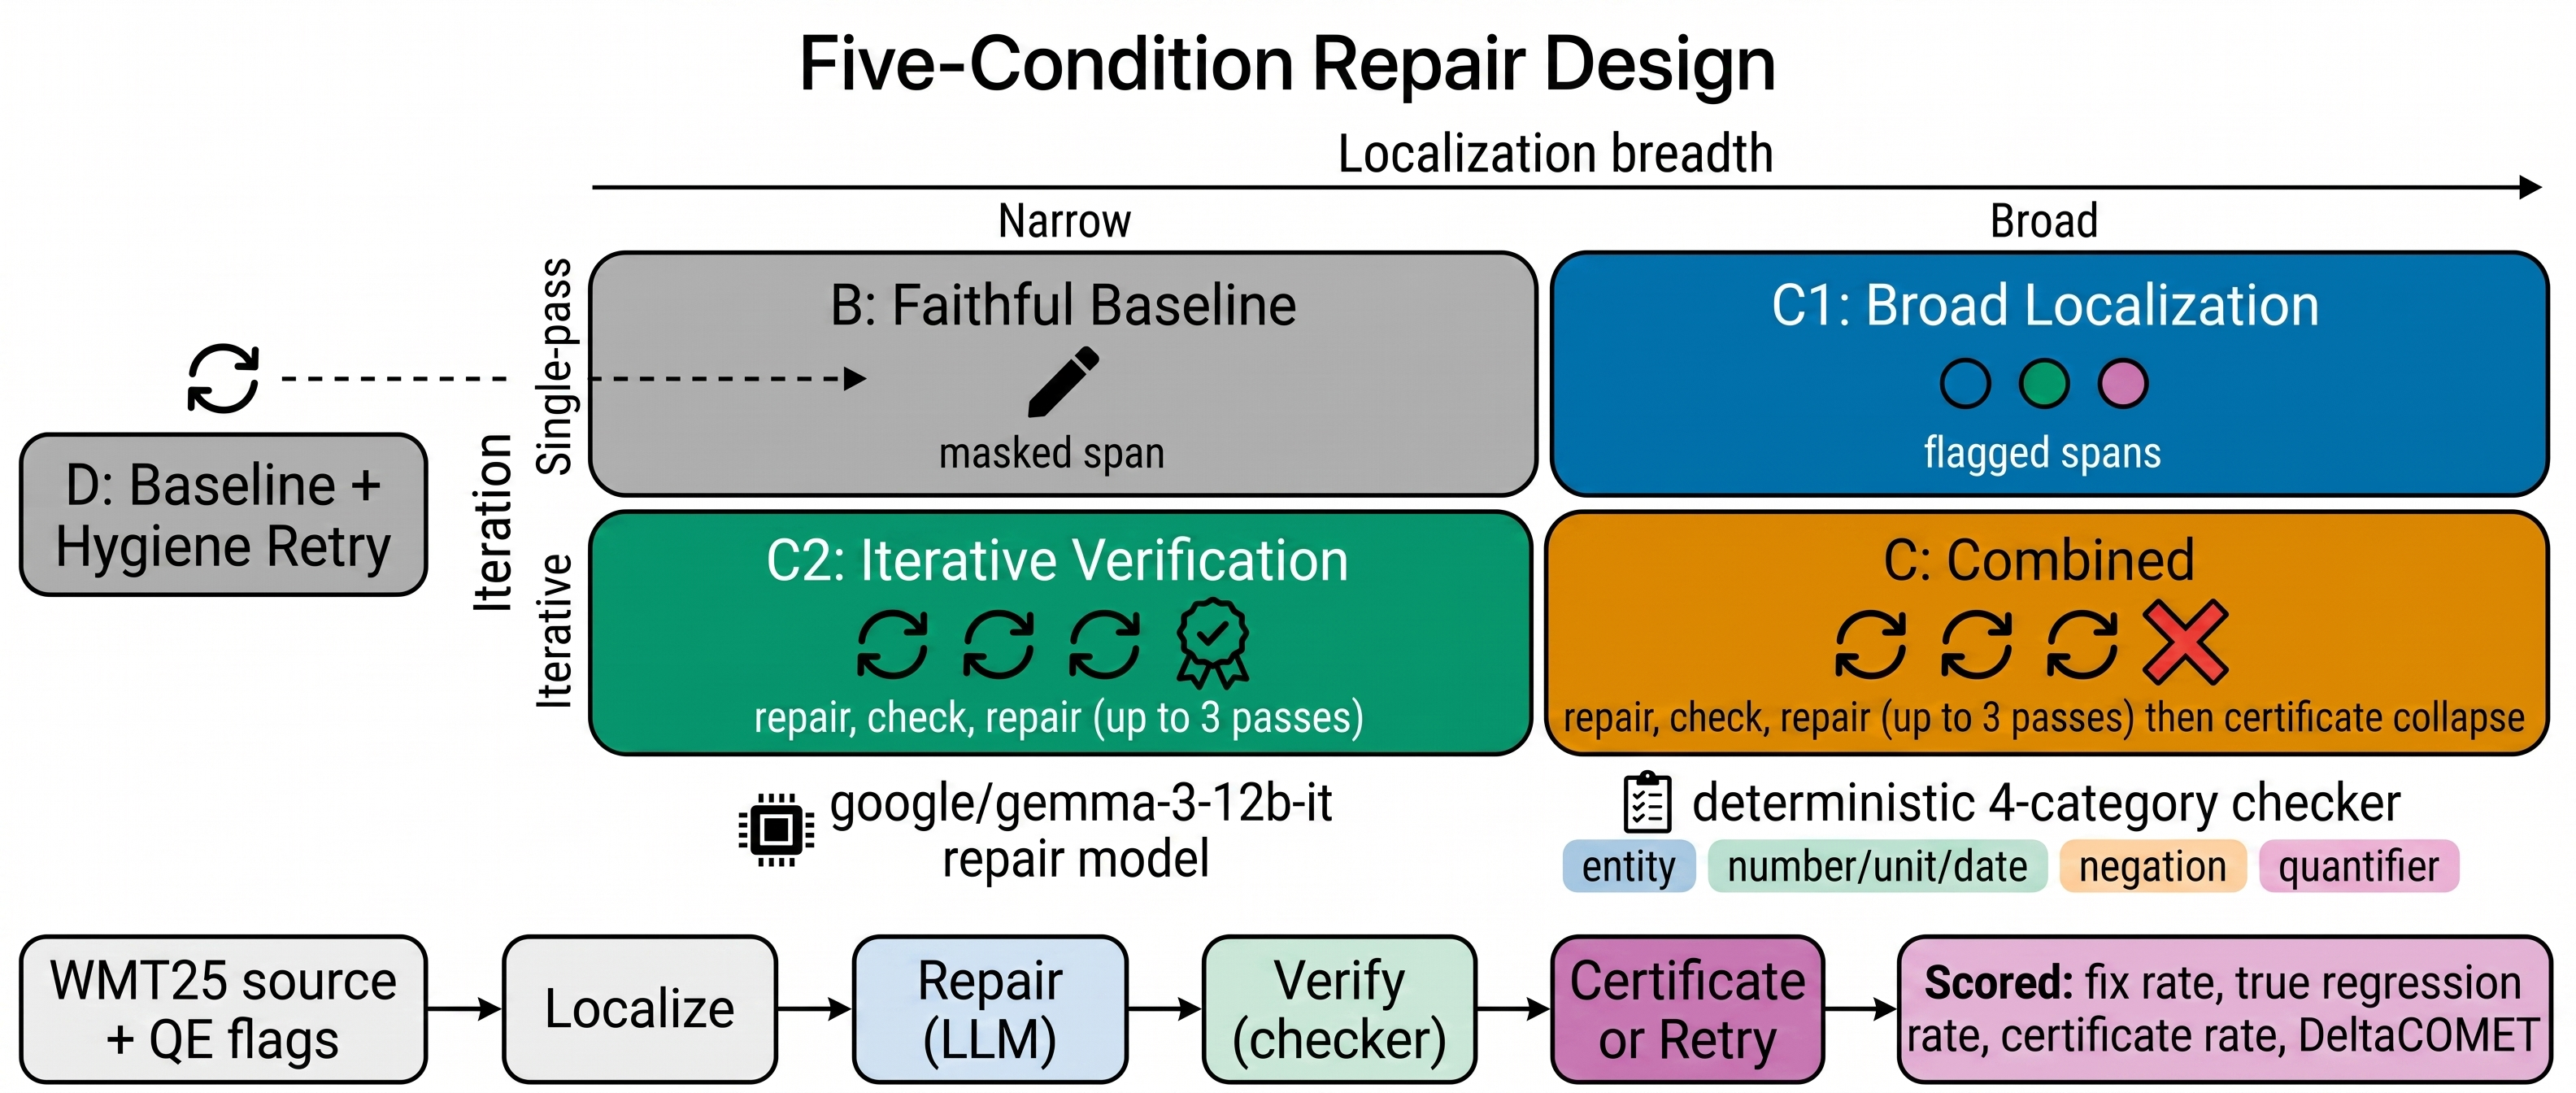
\includegraphics[width=\linewidth,height=0.85\textheight,keepaspectratio]{figures/fig1_v0.jpg}
  \caption{The five-condition factorial design used throughout this protocol. B (faithful masked-fill baseline) and D (B plus hygiene retry) use narrow, single-pass repair with no checker. C1 broadens localization to a whole-sentence deterministic content-invariant checker but repairs in a single uncorrected pass. C2 keeps narrow, QE-span-only localization but iterates repair-and-reverify against the checker up to a three-pass budget. Condition C combines both changes: broad checker-driven localization plus iterative repair-and-reverify up to the same three-pass budget, stopping on a zero-flag certificate.}
  \label{fig:fig1}
\end{figure}

Figure~\ref{fig:fig1} lays out the full design: the four-cell localization-by-iteration factorial plus the hygiene-only control, the shared repair model and checker, and the metrics each condition is scored on.

\section{Related Work}

\textbf{Quality-estimation-informed post-editing.} Automatic post-editing systems that use word-level QE as a training signal jointly train an encoder-decoder that regenerates the full target sentence in every variant; adding the QE signal reduces over-correction (18.30 vs. 19.39 TER) but never freezes a QE-clean span, so the model can still rewrite text no error was ever flagged in \citep{Deoghare2023}. A later system replaces the auxiliary-signal approach with Grid Beam Search, forcing QE-tagged ``OK'' spans as lexical constraints while the decoder keeps freedom to reorder and rephrase around them; this is closer to scoped editing in spirit but is a soft constraint on regeneration rather than a frozen, iteratively verified span, and the paper's own oracle-versus-predicted-tag gap of 0.3--1.3 TER shows the method's ceiling is set by QE tag accuracy without isolating that dependency as a separate factor \citep{Deoghare2025}. Prompting large language models directly with structured error annotations improves post-editing outcomes over unstructured feedback, but every condition in that study still regenerates the sentence and none tests a repair-then-verify loop against a single-pass repair with the same signal \citep{Ki2024}. A related line automatically predicts MQM-style error spans and post-edits with them inside an LLM-as-judge evaluation pipeline, again as a one-shot correction step \citep{Lu2024}. A third WMT25 Task 3 submission generates a natural-language explanation of each QE-flagged error with the xTower explanation model and hands that explanation to a large language model as the correction prompt \citep{Sharma2025}; like every system reviewed here, it regenerates the flagged segment in a single pass with no re-verification step.

\textbf{Localization breadth as a standalone factor: the closed EAMT 2026 lead.} A prior iteration's targeted literature search left one candidate unfetched: ``Smarter edits? Post-editing with error highlights and translation suggestions'' (EAMT 2026), flagged as its top open item because the abstract suggested it might vary highlight breadth across conditions. This iteration fetches the paper in full and classifies it against the same four-way decision rule (separates the factors / bundles the factors / varies only one factor / out of scope) used for the six previously checked candidates \citep{vanTellingen2026}. The paper studies four human-post-editing conditions for professional English-Dutch translators -- unassisted editing, QE-derived highlights from xCOMET-XXL spans, APE-derived highlights obtained by Levenshtein-diffing the raw MT output against a single xTower-Instruct-13B correction pass, and the same APE spans shown together with the correction text itself -- and confirms, via quoted methods text, that xTower is invoked exactly once per sentence in every condition: one scoring pass feeds one correction pass, reused post-hoc by the two highlight-derived conditions. A full-text regex sweep for iteration language returns exactly two matches, both to ``repeated measures ANOVA,'' a statistical test design unrelated to repeated correction attempts. Localization breadth does vary -- QE-derived spans are narrower, sometimes single characters, while diff-derived spans are broader and score higher against human oracle edits -- so the paper varies only one factor, with no iteration axis present in any condition. It is also, independently of that finding, a human-translator productivity study (keystrokes, editing time, satisfaction surveys) rather than an automated repair-loop study measuring fix rate, regression rate, or $\Delta$COMET, so it is not attempting the same measurement this project's protocol makes. With this candidate closed, the search now covers seven candidates in total -- TEaR, two WMT25 Task 3 submissions, xTower, SSPO, TranslationCorrect, a non-MT self-localization paper, and this EAMT 2026 study -- none of which independently varies both localization breadth and iteration/re-verification as two separately measured factors while holding the other fixed. TEaR remains the closest prior ablation: it runs an estimate-and-refine loop for LLM-based machine translation and reports an explicit ablation over the number of refinement rounds, one through five, holding its estimation mechanism fixed across every round \citep{Feng2025}. Its own Appendix D experiment on WMT23 Chinese-English finds that repeated iteration can \emph{hurt} translation performance relative to a single round -- a one-dimensional, iteration-only finding that varies the same factor Condition C2 isolates, but never varies localization breadth as a second, separately controlled factor. On the strength of this now-closed search, we state this paper's novelty claim without qualification: we are not aware of prior work in machine-translation automatic post-editing or scoped span editing that holds localization breadth and iteration apart as two independently varied, separately measured factors the way this protocol's C1-vs-C2-vs-C design does, though TEaR's iteration-count ablation independently supports this paper's own finding that more refinement rounds do not monotonically help, from a design that never tested whether broadening what is checked changes that picture.

\textbf{Localized and energy-guided editing.} Locate-and-edit approaches to controlled text generation obtain a full generation from a base model, then use an energy function to find and replace only the spans that violate a stated constraint, explicitly to avoid the semantic drift full regeneration under a constraint tends to introduce \citep{Son2024}. This is the closest existing mechanism to the localization half of our design, but it has not been applied to machine translation and has not been evaluated with localization breadth and iteration held apart as separately controlled factors.

\textbf{Iterative self-refinement.} Self-Refine shows that a single language model can generate an output, critique its own output, and revise it over several rounds without external supervision, improving results on tasks from code optimization to dialogue response generation \citep{Madaan2023}. Condition C2 and Condition C both iterate against a deterministic, non-learned checker rather than the repair model's own judgment, precisely to avoid the known unreliability of a model critiquing its own errors. Our results now complicate the general expectation that more refinement rounds monotonically help in three distinct ways, sharper than before: C2 shows iteration against an external, deterministic verifier reliably fixes the specific things the verifier checks without improving a downstream metric it was never checking; Condition C shows that broadening what the verifier checks, inside the same fixed-budget iteration loop, makes the loop worse at the very thing it is meant to guarantee -- a verified, certified output; and, newly this iteration, Condition C's now-real $\Delta$COMET shows that broadening plus iterating also fails to recover the whole-sentence quality gain broadened localization achieves on its own, closing the one axis that remained open when only correctness had been measured.

\textbf{Counterexample-guided synthesis.} Counterexample-Guided Inductive Synthesis (CEGIS) is a synthesis loop in which a candidate is checked against a specification by a verifier that either certifies it or returns a concrete counterexample scoping the next candidate, terminating on an explicit certificate rather than a fixed budget \citep{Jha2015}. We do not claim to import CEGIS as a synthesis algorithm; our checker's ``counterexample'' is a flagged span, not a candidate-generalizing constraint, and nothing in our design performs unrealizability reasoning or generalizes across counterexamples. What we borrow is narrower -- the separation of concerns between what a verifier is allowed to see (localization breadth) and whether the loop runs more than once (iteration). Condition C's collapsed certificate rate under a fixed pass budget is a concrete illustration of exactly the risk CEGIS's certificate-or-counterexample loop is designed around: a budget-capped loop that broadens its own checked surface can spend its entire budget without ever reaching the certificate state CEGIS treats as the only acceptable termination condition. This iteration's precision-stratified analysis (Section 6.7) sharpens that illustration: the collapse is not spread evenly across the checker's tracked invariants but concentrates where the checker's own precision is lowest, suggesting the risk CEGIS is built around compounds with a second, independent risk -- an imperfect verifier that keeps re-issuing counterexamples against invariants it was never actually violating.

\textbf{Evaluation infrastructure.} All $\Delta$COMET figures in this paper, for every one of the five conditions, are now computed with the same reference-free quality-estimation checkpoint the shared task uses, \texttt{wmt22-cometkiwi-da} \citep{Rei2022}. Our natural-error data is WMT25 Task 3's released test set \citep{Lavie2025}; our injected-error data is built from WMT24++, a disjoint, human-post-edited multilingual corpus spanning 55 languages and dialects \citep{Deutsch2025}.

\section{Preliminaries}

We define four terms used throughout the protocol.

A \textbf{content invariant} is a piece of source-sentence meaning -- a named entity, a number, unit, or date, a negation polarity marker, or a quantifier -- that must survive translation, and that can be checked deterministically (via named-entity recognition, regular expressions, cue-word lists, or alignment) rather than judged by a learned model. We check four invariant categories: entity identity, number/unit/date value, negation polarity, and quantifier scope.

A translation's \textbf{certificate} is the state in which every content invariant extracted from its source sentence has been checked and passes. Conditions C2 and C stop iterating as soon as a repair passes the checker (certificate reached) or a fixed pass budget is exhausted, whichever comes first; \textbf{certificate rate} is the fraction of rows that reach this state within the budget, distinct from \emph{fix rate}, which credits a row whenever its specific ground-truth-corrupted invariant is repaired regardless of whether every other invariant in the sentence also passes. A certificate is computed only over the invariant categories the checker's own validation certifies as usable for the current run (Section 6.1); when a row's own known-corrupted category falls in an excluded cell, that row is neither dropped from the certificate-rate denominator nor scored on its own corruption, but is instead scored on whichever other, non-excluded invariants the checker does track in that sentence (Section 6.7 verifies this behavior directly against the code and against raw per-row logs).

\textbf{Localization breadth} is how much of the sentence a system is allowed to flag as needing repair. \emph{Narrow} localization repairs only the span the original quality-estimation model flagged (Conditions B, D, and C2); \emph{broad} localization repairs every invariant our checker finds violated, whether or not quality estimation flagged it (Conditions C1 and C).

\textbf{Iteration} is whether a flagged span, once repaired, is re-checked and re-repaired if it still fails, up to a fixed pass budget, or whether the system accepts a single repair pass unconditionally. Conditions B, D, and C1 use a single, uncorrected pass; C2 and C iterate.

\section{Method}

\subsection{Design Rationale}

Our method isolates localization from verification by construction: it fixes the repair model identically across every condition that performs a repair, and it varies localization breadth and iteration as two independently switchable factors rather than one bundled toggle, giving a two-by-two design (narrow/broad $\times$ single-pass/iterated) plus a hygiene-only control. Prior iterations established the two single-lever effects: broadening localization alone (C1) moves $\Delta$COMET substantially but costs fix rate and true regression rate; iterating alone, holding localization narrow (C2), recovers that correctness cost without moving $\Delta$COMET. Condition C -- both levers engaged at once -- completes the design's fourth cell. This iteration closes the one remaining gap in that completion: Condition C's quality-axis metric is now the same real checkpoint used everywhere else in the study, not a substitute proxy.

\subsection{Five Conditions, All Now Fully and Comparably Scored}

All five conditions share one deterministic content-invariant checker (Section 6.1) and, in every condition that performs a repair, one fixed repair model, \texttt{google/gemma-3-12b-it}. Conditions B, D, and C1 were executed in an earlier iteration; Condition C2 in the iteration after that; Condition C's repair sweep in the iteration after that; and this iteration performs a scoring-only rerun that obtains Condition C's real $\Delta$COMET, generating no new repair text and making no new repair-model calls.

\textbf{Condition B (faithful baseline).} A reproduction of the original masked-fill system: the QE model's flagged span is masked with a placeholder token according to the original system's severity-conditioned masking rule, filled with one repair-model pass, and accepted without any check \citep{Padmanabhan2025}.

\textbf{Condition D (hygiene filter, no checker).} Condition B, plus a trivial post-hoc filter that detects and retries any output containing a leftover mask token, garbled placeholder text, or leaked instruction-format text. No content-invariant checker is involved.

\textbf{Condition C1 (broad localization, single pass).} The checker flags every invariant violation in the sentence, not only the original QE span; each flagged violation is repaired in one uncorrected pass, with no re-verification. Per-category repair scope is gated by the checker's own validated precision and recall (Section 6.1): a (language, category) cell falling below 0.5 on either metric in the within-experiment validation is excluded from repair scope.

\textbf{Condition C2 (narrow localization, iterative verification).} Localization stays restricted to the original QE-flagged span, but that span is repaired, re-checked by the checker against the specific invariant categories it flags, and re-repaired with a targeted, checker-detail-scoped prompt if it still fails, up to a fixed three-pass budget, stopping as soon as the checker certifies the repair. This isolates the effect of iteration while holding localization fixed at narrow.

\textbf{Condition C (broad localization, iterative verification).} Both changes combined: the checker re-scans the entire current candidate text fresh on every pass, flagging every invariant violation it finds (not restricted to the row's own known-corrupted category, since Condition C's localization does not know in advance which category was corrupted), and each flagged violation is repaired and re-verified up to the same three-pass budget, stopping on a zero-flag certificate. This condition tests whether broadened localization's quality gain and iteration's correctness gain can be obtained together.

C2 and C were built by extending the checker module and OpenRouter client from the B/D/C1 artifact verbatim, so all five conditions share an identical checker, repair model, and API client. C2 and C regenerated the same stratified 320-natural/240-injected-pool row population using the same seed and stratification rule as B/D/C1, and row-ID identity against the prior run's logged row selection was verified true for all three subsets (natural, injected-pool, injected-heldout) before any comparison was trusted -- including, this iteration, a direct byte-identity check between B/D/C1's and Condition C's own selections, which had never been cross-checked directly before.

\subsection{Condition C's Quality-Axis Rescue}

The prior iteration's Condition C run could not download the real \texttt{wmt22-cometkiwi-da} checkpoint: Hugging Face Hub returned HTTP 429 on all twelve retry attempts across two separate multi-minute backoff probes, forcing a substitute, non-comparable proxy metric. This iteration runs a scoring-only rerun over Condition C's already-generated 320 natural-row repair outputs -- no new repair generation, no new repair-model calls -- using genuinely new mitigations against the recurring failure: an alternate mirror endpoint (\texttt{hf-mirror.com}) as a fallback path, and download attempts spread across real wall-clock-separated windows (offsets of 0, 25, 75, and 165 minutes) rather than in-process exponential backoff, which had not addressed the persistent, not transient, nature of the prior failure\footnote{Code: \url{https://github.com/ai-inventor-papers/ai-invention-e9bf19-isolating-what-fixes-failed-span-editing/tree/main/round-5/experiment-1}}. Both Condition C's and Condition B's source artifacts were located on disk via content-signature verification -- unique metadata keys and exact row counts -- rather than a hardcoded path, so the script fails loudly with a blocking assertion if either cannot be found, rather than silently scoring the wrong repair outputs.

On this run, the real checkpoint downloaded successfully on the very first attempt: window offset zero, the primary \texttt{huggingface.co} endpoint, 0.26 seconds, a single log entry, no 429. The prior throttling was not reproduced. The \texttt{wmt22-cometkiwi-da} XLM-R-based quality-estimation model then scored all 320 pre-repair and 320 post-repair texts on GPU, the identical scoring procedure used for B, D, C1, and C2. A fully-coded fallback path -- reusing Condition B's own LLM-judge proxy configuration verbatim, for a same-proxy, same-run comparison, exactly as the prior review round's mitigation critique recommended as a fallback -- was implemented but never needed to execute, since the real checkpoint was obtained directly.

\section{Data}

We reuse, without modification, the complete data construction validated in an earlier iteration: 6,000 natural WMT25 Task 3 rows across six English-source language pairs and five domains, carrying the QE model's released flagged spans and severity labels \citep{Lavie2025}; and 2,519 injected-error rows built by programmatically corrupting clean WMT24++ target text into one of four invariant categories (named-entity swap, number/unit/date alteration, negation polarity flip, quantifier substitution), each carrying the pre-corruption text, the corrupted text, and the exact character span of the change so a checker's precision and recall against a known answer is computable directly \citep{Deutsch2025}. Both groups are split by language pair (and, for the injected set, by category) into an experimental pool and a checker-validation holdout kept strictly disjoint from it.

All five conditions run on the same 320 natural and 240 injected-pool rows, from the same two language pairs (en-ru\_RU, en-uk\_UA). This iteration's contribution to the data pipeline is again verified reuse rather than new construction: no new rows were sampled, no new repairs were generated, and the rescored Condition C repair outputs are the identical text objects scored by the prior iteration's proxy metric, now scored a second time with the real checkpoint instead.

$\Delta$COMET for all five conditions in this protocol is now computed with \texttt{wmt22-cometkiwi-da}, the same checkpoint the shared task's organizers use as the exact scorer behind every entry in its results table \citep{Rei2022,Lavie2025}. This closes the metric-comparability gap that limited the prior iteration's Condition C reporting to a directionally-suggestive proxy.

\section{Results}

This iteration performs two kinds of work: a scoring-only rescue of Condition C's quality axis onto the same real checkpoint every other condition uses, and a set of re-analyses of already-computed results that respond directly to three reviewer critiques of the certificate-rate mechanism, the checker-eligibility scope of the paper's headline comparison population, and a normal-approximation bias-direction claim. No new repair text was generated and no new LLM repair calls were made in either. We report the full, now-comparable B/D/C1/C2/C scorecard first, then the three targeted re-analyses.

\subsection{Reconciling Two Checker-Validation Tables}

The checker's validity was measured twice in this project, at different scopes. The \emph{global} table scores the checker against all 448 injected and 1,080 natural rows in the checker-validation holdout, across all six languages and four categories, using a natural-row precision proxy (any checker flag on a natural row that does not overlap a sparse QE-flagged span counts as a false positive, a noisy and conservative signal). The \emph{within-experiment} table scores the checker against only the 175-row subset of that holdout actually available for the two language pairs this experiment runs on, using an exact single-positive-per-row precision against known ground-truth corruption spans on injected rows only -- a stricter, directly interpretable metric that is the one that actually gates C1's and Condition C's repair scope.

\begin{table}[!htbp]
\centering
\small
\begin{tabular}{llccc}
\toprule
Language & Category & Global $P$ / $R$ & Within-exp $P$ / $R$ & Usable (within-exp) \\
\midrule
ru\_RU & named\_entity & 0.039 / 1.000 & 0.324 / 1.000 & No \\
ru\_RU & number\_unit\_date & 0.184 / 1.000 & 0.575 / 1.000 & Yes \\
ru\_RU & negation\_polarity & 0.867 / 0.565 & 0.857 / 0.522 & Yes \\
ru\_RU & quantifier\_scope & 0.152 / 1.000 & 0.591 / 0.565 & Yes \\
uk\_UA & named\_entity & 0.029 / 0.696 & 0.370 / 0.696 & No \\
uk\_UA & number\_unit\_date & 0.132 / 1.000 & 0.575 / 1.000 & Yes \\
uk\_UA & negation\_polarity & 0.824 / 0.609 & 0.778 / 0.609 & Yes \\
uk\_UA & quantifier\_scope & 0.197 / 1.000 & 0.500 / 0.429 & No \\
\bottomrule
\end{tabular}
\caption{The two checker-validation procedures, restricted to the eight (language, category) cells this experiment runs on. $P$ is precision, $R$ is recall; usability requires both $\geq 0.5$.}
\label{tab:checkervalidation}
\end{table}

Three cells fail the within-experiment threshold and are excluded from C1's and Condition C's repair scope: ru\_RU and uk\_UA named-entity, and uk\_UA quantifier-scope. \textbf{The eligible five cells -- ru\_RU number/unit/date, ru\_RU negation-polarity, ru\_RU quantifier-scope, uk\_UA number/unit/date, and uk\_UA negation-polarity -- are what actually make up the ``checker-eligible'' population used later in this section (Section 6.7); we state this here, at first mention of the checker's usability gate, rather than only in a table caption after the headline comparison has already been made, per a reviewer critique of the prior draft.} Condition C's own checker validation, run fresh against the same 175-row holdout this iteration, reproduces this table's within-experiment precision and recall values for the number/unit/date and quantifier categories exactly (e.g. ru\_RU quantifier-scope precision 0.591/recall 0.565), but its named-entity cells drifted to precision/recall exactly $0.0/0.0$ in Condition C's own execution environment (versus this table's ru\_RU $0.324/1.000$ and uk\_UA $0.370/0.696$) -- named-entity detection is effectively inert in Condition C's run, a drift documented directly in Section 6.7 and confirmed not to change the excluded-cell set, since named-entity already fails the threshold under both readings.

\subsection{Condition-B Fidelity}

Before trusting any comparison built on the substitute repair model, this protocol pre-registered a quantitative tolerance for Condition B's reproduction of Padmanabhan (2025)'s $-0.0108$ mean $\Delta$COMET: the measured value must share Padmanabhan's sign, and its magnitude ratio to the original must fall in $[0.5\times, 2.0\times]$. Condition B's pooled $\Delta$COMET is $-0.0164$ (95\% CI $[-0.0237,-0.0101]$), matching Padmanabhan's sign with a magnitude ratio of $1.52\times$ -- inside the tolerance band, close enough to its edge that we report this a borderline pass rather than an unqualified one.

\subsection{The Full Five-Condition Comparison}

Negation-polarity corruptions in the injected set are span \emph{deletions} (the corrupted span is empty), so narrow-localization conditions (B, D, C2) structurally cannot attempt a negation repair at all -- fix\_success is trivially false for 100\% of these rows by construction, not because of a repair-quality failure -- while broad-localization conditions (C1, C) can attempt them because their checker scans the whole sentence rather than masking a specific span. Every fix-rate and true-regression-rate figure below is reported pooled \emph{excluding} the 60 structurally-unattemptable negation rows (180 rows, the population every condition can genuinely attempt), the common basis used across every table in this paper.

\begin{figure}[!htbp]
  \centering
  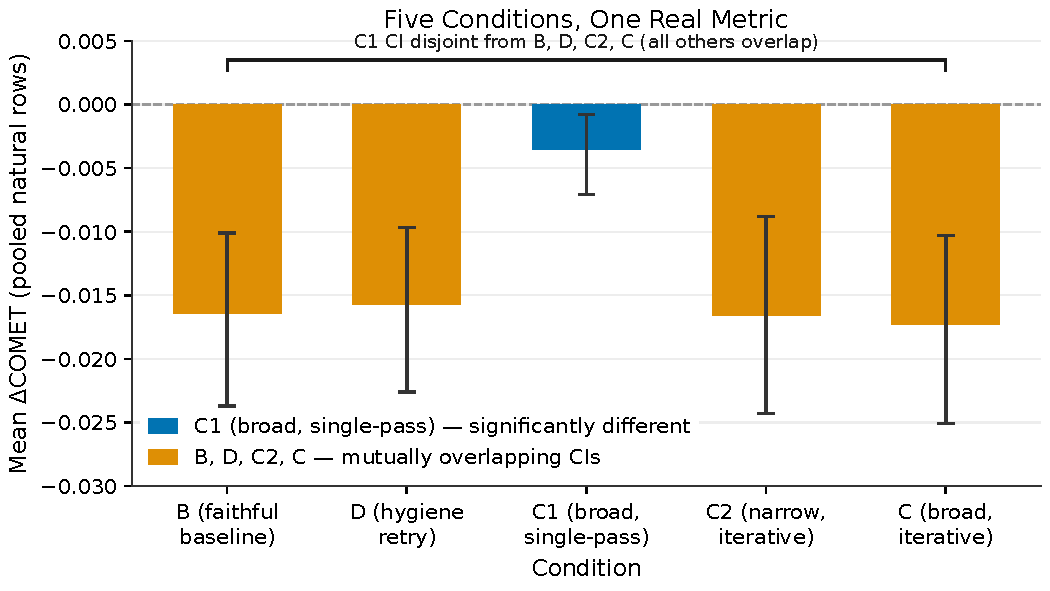
\includegraphics[width=\linewidth,height=0.85\textheight,keepaspectratio]{figures/fig2_v0.pdf}
  \caption{Mean $\Delta$COMET (pooled natural-row sample, both language pairs) for all five conditions, all now scored on the identical real \texttt{wmt22-cometkiwi-da} checkpoint. Error bars are 95\% bootstrap confidence intervals. Condition C's interval overlaps B's and C2's almost completely and does not overlap C1's at all: combining both repair levers does not recover broadened localization's quality gain.}
  \label{fig:fig2}
\end{figure}

Table~\ref{tab:fivecond} places every condition side by side, now with $\Delta$COMET for Condition C computed on the same real checkpoint as the other four conditions -- the single largest change from the prior iteration.

\begin{table}[!htbp]
\centering
\small
\begin{tabular}{lcccccc}
\toprule
Condition & $\Delta$COMET (pooled, real ckpt) & Fix rate & True regr. rate & Certificate rate & Edit vol. & LLM calls/sent. \\
\midrule
B & $-0.0164$ (CI $[-0.0237,-0.0101]$) & 0.9833 & 0.0667 & n/a & 0.146 & $\sim$1.0 \\
D & $-0.0157$ (CI $[-0.0226,-0.0097]$) & 0.9833 & 0.0667 & n/a & 0.146 & $\sim$1.0 \\
C1 & $-0.0035$ (CI $[-0.0071,-0.0008]$) & 0.6056 & 0.1389 & n/a & 0.021 & 0.85 \\
C2 & $-0.0166$ (CI $[-0.0243,-0.0088]$) & 0.9889 & 0.0722 & 0.917 & 0.164 & 2.29 \\
C & $-0.0173^{\dagger}$ (CI $[-0.0251,-0.0103]$) & 0.6278 & \textbf{0.2167} & \textbf{0.267} & 0.022 & 2.53 \\
\bottomrule
\end{tabular}
\caption{Complete five-condition scorecard, all $\Delta$COMET values now on the identical real \texttt{wmt22-cometkiwi-da} checkpoint. Fix rate, true regression rate, and edit volume are pooled excluding negation-deletion rows, the population every condition can attempt; $\Delta$COMET is pooled over the natural-row sample, both language pairs. $^{\dagger}$Condition C's $\Delta$COMET is a scoring-only rerun of the already-generated repair outputs, obtained this iteration after the prior iteration's checkpoint-access failure was not reproduced. n/a marks conditions with no certification loop. Bold marks Condition C's regression rate and certificate rate, the two values that most directly disconfirm the combined-condition hypothesis.}
\label{tab:fivecond}
\end{table}

Condition C's real $\Delta$COMET is $-0.0173$, with a 95\% confidence interval that overlaps B's ($-0.0164$) and C2's ($-0.0166$) almost entirely, and does not overlap C1's ($-0.0035$, CI upper bound $-0.0008$) at all. Broken out by language pair, the pattern holds: en-ru\_RU $-0.0228$ ($n=160$) and en-uk\_UA $-0.0117$ ($n=160$), both closer in magnitude to B's per-pair figures than to C1's. This resolves what was the paper's one remaining open question: combining broadened localization with iteration does not recover broadened localization's quality gain either. Every axis this protocol measures -- fix rate, true regression rate, certificate rate, and now $\Delta$COMET -- tells the same story: Condition C is not intermediate between C1 and C2, and it is not additive; on $\Delta$COMET specifically, it lands statistically indistinguishable from the unedited faithful baseline, meaning the whole-sentence quality benefit that broadened localization achieves on its own (C1) is entirely lost once iteration is added on top of it.

C2's correctness metrics essentially match the simplest narrow-localization baselines: fix rate 0.9889 against B/D's 0.9833, true regression rate 0.0722 against B/D's 0.0667. What C2 dramatically improves on is C1: relative to C1's single-pass broadened localization, C2's narrow-but-iterated approach lifts fix rate by roughly 0.38 points on this excluding-negation basis and lowers true regression rate by 0.07 points, both differences confirmed by a true paired bootstrap on the 180 matched rows (true-regression-rate difference $0.0667$, 95\% CI $[0.0111,0.1278]$, excluding zero). $\Delta$COMET moves the other way: C2's pooled $\Delta$COMET ($-0.0166$) is statistically indistinguishable from B and D, and a paired comparison against C1 on the same matched rows (using a documented normal-approximation substitute, formalized and its direction now proven in Section 6.9) puts the C1-minus-C2 difference at $0.0131$ (95\% CI $[0.0047,0.0214]$, excluding zero in the direction that C1 is better). Iteration is the load-bearing mechanism for recovering correctness, holding localization narrow; broadened localization, not iteration, is what single-lever evidence has shown moves whole-sentence quality -- and Condition C's now-comparable $\Delta$COMET shows that combining the two levers does not transfer that quality gain across.

\subsection{Why the Certificate-Rate Collapse Happens: A Precision-Stratified Re-Analysis}

\begin{figure}[!htbp]
  \centering
  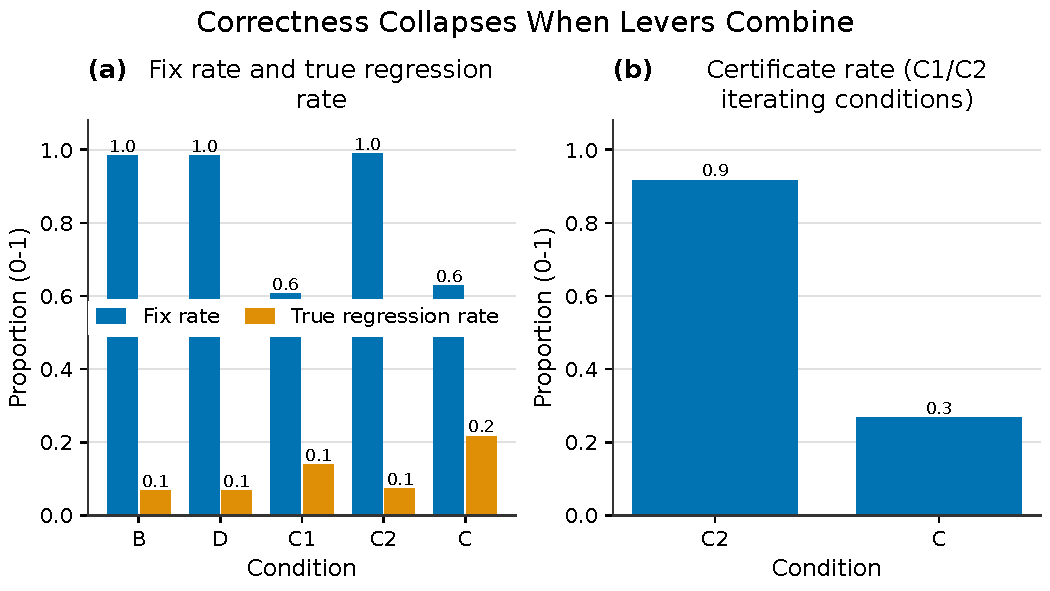
\includegraphics[width=\linewidth,height=0.85\textheight,keepaspectratio]{figures/fig3_v0.pdf}
  \caption{Fix rate, true regression rate, and certificate rate across the five conditions (pooled excluding negation-deletion rows, 180 rows; certificate rate n/a for B, D, C1 which have no verification loop). Condition C's true regression rate is the highest of all five conditions and its certificate rate is the lowest of the two iterating conditions, despite sharing C1's checker and C2's iteration budget.}
  \label{fig:fig3}
\end{figure}

The prior draft attributed Condition C's certificate-rate collapse (0.917 in C2, once localization broadens to match C1's scope, to 0.267 in C) to a repair that fixes the invariant it targeted while leaving -- or introducing -- a violation elsewhere in the sentence that the next pass must also address. A reviewer of that draft pointed out this attributes the collapse entirely to genuine cross-invariant damage, when the checker's own validated precision on usable cells (Table~\ref{tab:checkervalidation}) ranges from 0.575 to 0.857 -- meaning a substantial share of the checker's re-flags on already-correct repairs could themselves be false positives, and that number\_unit\_date's own pattern (highest fix rate of any category at 0.983, but the lowest certificate rate at 0.067 and the highest mean pass count at 2.90, near the three-pass cap) is equally consistent with checker-noise-driven churn as with genuine new damage.

This iteration answers the question the reviewer's critique actually poses: is the collapse uniform across the checker's precision levels (favoring the genuine-damage story) or concentrated where checker precision is lowest (favoring the checker-noise story)? Table~\ref{tab:checkervalidation}'s five usable cells split into a high-precision tier (negation\_polarity, precision 0.78--0.86 across both languages) and a low-precision tier (number\_unit\_date and quantifier\_scope, precision 0.575--0.65). Recomputing Condition C's per-cell certificate rate directly from raw per-row logs -- validated as an exact superset of Condition C's own pre-aggregated category table, and additionally recovering negation\_polarity's certificate rate, which that table left null -- gives a mean certificate rate of $0.35$ in the high-precision tier ($n=2$ cells: ru\_RU $0.3667$, uk\_UA $0.3333$) against $0.089$ in the low-precision tier ($n=3$ cells: ru\_RU number\_unit\_date $0.0333$, ru\_RU quantifier\_scope $0.1333$, uk\_UA number\_unit\_date $0.100$) -- a $3.9\times$ ratio, with the collapse pattern classified \texttt{concentrated\_in\_low\_precision\_tier}.

\begin{figure}[!htbp]
  \centering
  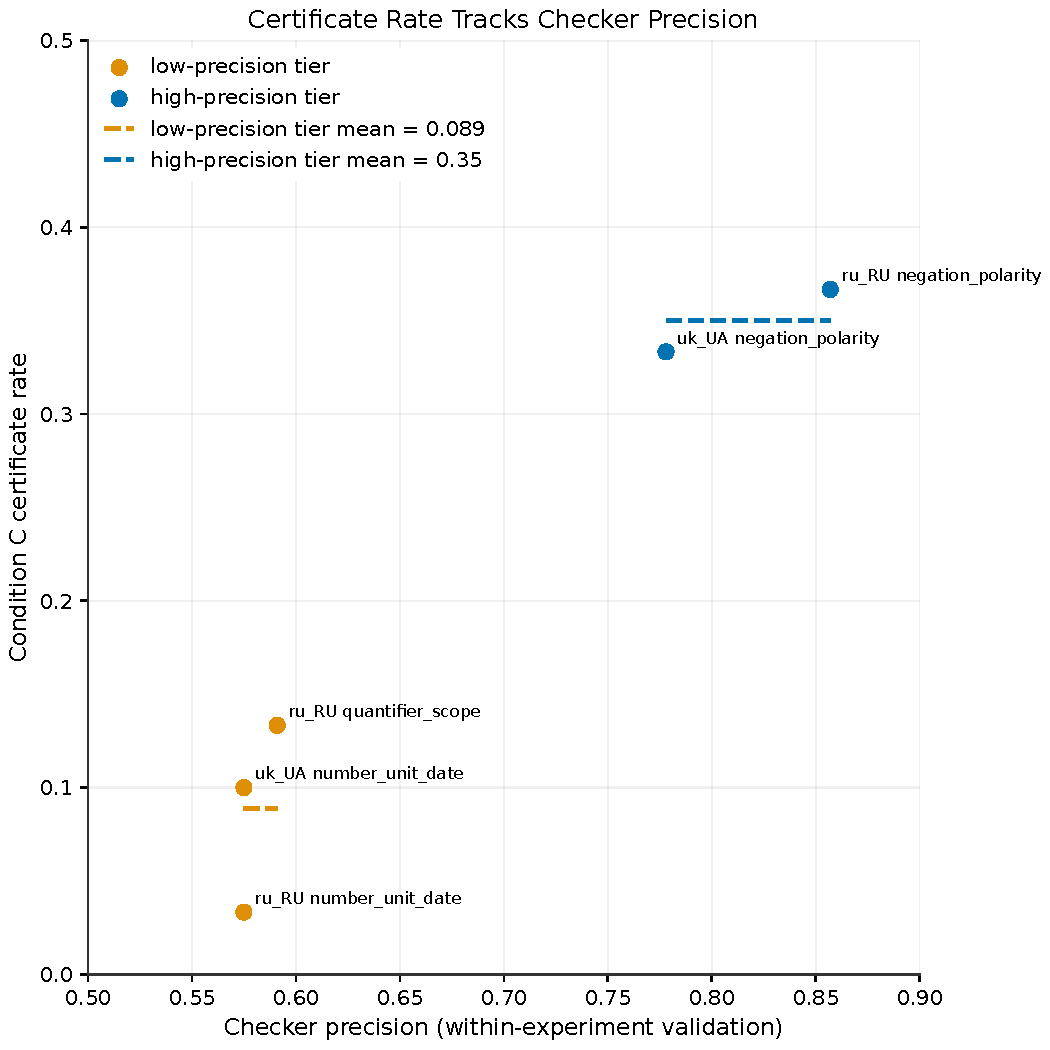
\includegraphics[width=\linewidth,height=0.85\textheight,keepaspectratio]{figures/fig4_v0.pdf}
  \caption{Condition C's certificate rate per (language, category) cell, plotted against that cell's own checker precision from Table 1's within-experiment validation. The two negation\_polarity cells (highest checker precision, 0.78--0.86) reach a mean certificate rate of 0.35; the three number\_unit\_date and quantifier\_scope cells (lowest checker precision, 0.575--0.65) reach only 0.089, a 3.9$\times$ gap consistent with -- though not proof of -- checker-noise-driven re-flagging.}
  \label{fig:fig4}
\end{figure}

This is consistent with checker-noise-driven churn concentrating certificate failure where the checker's own detection precision is lowest, rather than a uniform cross-invariant regression spread evenly across every checked category. We report it exactly that way and no further: the analysis does not prove checker noise is the sole or even dominant cause, and it does not distinguish a noise-driven mechanism from a genuinely harder-to-satisfy invariant class that happens to also have lower checker precision -- number\_unit\_date and quantifier\_scope require an exact numeric or scope match to certify, which is plausibly just harder to repair correctly regardless of how noisy the checker's flags are. The two explanations are confounded in this data and cannot be separated without an independent measure of true repair difficulty per category, something no artifact in this project computes. The sample is also small: five usable cells split two against three across tiers is not enough to support a confident causal conclusion, and we flag this explicitly rather than letting the $3.9\times$ ratio read as more decisive than it is. No fourth, widened-pass-budget artifact with per-pass false-positive tracking exists among this iteration's actual dependencies, so this precision-tier estimate is the best available first-order signal, not a supplementary check on a stronger one -- and the next iteration's proposed budget-widening experiment (Discussion) is the natural way to obtain that stronger evidence.

\subsection{Does the Headline Ordering Survive Restriction to Fully Checker-Eligible Cells?}

A second reviewer critique observed that Table~\ref{tab:fivecond}'s 180-row ``every condition can attempt'' population implicitly pools cells the checker can and cannot actually localize and verify: named\_entity is excluded from repair scope in both tested languages, and quantifier\_scope is excluded in uk\_UA, so C1's and Condition C's named-entity repairs in that pooled figure rely on the original QE-flagged span rather than the broadened checker's own localization, despite being counted as ``broad localization'' evidence.

We re-derive the checker's eligibility scope directly from Table~\ref{tab:checkervalidation}'s own recall $\geq 0.5$ AND precision $\geq 0.5$ threshold rule rather than restating it from memory, and find it is in fact wider than the plan text's own prior restatement: five of the eight (language, category) cells pass the threshold, not three -- negation\_polarity clears the bar in \emph{both} languages (ru\_RU $0.857/0.522$, uk\_UA $0.778/0.609$), a cell the earlier restatement had omitted. Restricting every condition to exactly these five eligible cells (150 of the 240 injected-pool rows, at a matched $n=150$ across all five conditions) gives Table~\ref{tab:eligible}.

\begin{table}[!htbp]
\centering
\small
\begin{tabular}{lccc}
\toprule
Condition & Fix rate (5 eligible cells) & True regr. rate (5 eligible cells) & Certificate rate (5 eligible cells) \\
\midrule
B & 0.5800 & 0.0400 & n/a \\
D & 0.5800 & 0.0400 & n/a \\
C1 & 0.5400 & 0.0800 & n/a \\
C2 & 0.9778 & 0.0556 & 0.9222 \\
C & 0.9333 & 0.1600 & 0.1933 \\
\bottomrule
\end{tabular}
\caption{All five conditions restricted to the five (language, category) cells that pass Table~\ref{tab:checkervalidation}'s own usability threshold (150 of 240 injected-pool rows, matched $n$ across every condition). The headline ordering -- C1's true regression rate exceeding C2's, Condition C's true regression rate the highest of the five, and certificate rate collapsing from C2 to C -- survives this restriction unchanged in direction.}
\label{tab:eligible}
\end{table}

Every headline comparison this paper makes survives the restriction: C1's true regression rate (0.0800) still exceeds C2's (0.0556); Condition C's true regression rate (0.1600) is still the highest of any condition on this restricted population, exceeding C1's by twice and C2's by nearly threefold; and certificate rate still collapses from C2's 0.9222 to C's 0.1933. Magnitudes shift, as expected -- Condition C's fix rate actually rises to 0.9333 on this restricted population, because it now excludes named\_entity, the category where C performs worst (Table~\ref{tab:categorybreakdown} below), leaving mostly number\_unit\_date, where C achieves near-total fix rate but the lowest certificate rate of any category. This confirms the restriction is not merely diluting the picture in one direction: fix rate improves for C while true regression rate and certificate rate still point in the same disconfirming direction as the full pooled comparison. The pattern this paper reports is not an artifact of pooling contested and uncontested checker cells together.

\subsection{What ``Certificate'' Means for an Excluded-Category Row}

A third, minor reviewer point asked what it means for a named\_entity\_swap row to reach a ``verified, zero-flag certificate'' when named\_entity is itself excluded from the checker's repair scope for both tested languages (Table~\ref{tab:checkervalidation}) -- Table~\ref{tab:categorybreakdown} (previously Table 3) reported a 0.500/0.533 certificate rate for that category without stating how it is computed. We answer this directly against the code and the raw per-row logs rather than by inference: Condition C's method builds its checker with the current run's excluded-cell set and calls it with exclusions respected, so an excluded (language, category) pair is never flagged at all, in either direction, for any row -- independent of whether that row's own known corruption falls in the excluded category. A row's certificate status is therefore computed only over the invariant categories the checker actually tracks for the current run's non-excluded cells; a named\_entity\_swap row is scored on whether the \emph{other} tracked invariants (number\_unit\_date, negation\_polarity, and quantifier\_scope where not itself excluded) are clean, never on whether its own named-entity corruption was fixed. A worked example row (\texttt{injected\_error\_augmentation:1215}, en-ru\_RU, named\_entity\_swap, certificate not achieved after three passes) confirms this directly: its logged flag categories across all three passes are \texttt{number\_unit\_date} and \texttt{quantifier\_scope} only, never \texttt{named\_entity}. Checking every named-entity row in the injected pool confirms the pattern holds without exception: named\_entity is never among the flagged categories for any row, in any pass, anywhere in Condition C's execution.

This same re-check surfaced an incidental finding, reported for completeness rather than because it changes any headline result: Condition C's own re-fit checker validation on the injected-heldout fold shows named\_entity recall and precision of exactly $0.0/0.0$ in both languages this run, versus $1.000/0.324$ (ru\_RU) and $0.696/0.370$ (uk\_UA) in the original B/D/C1 checker-validation run -- named-entity detection is effectively inert in Condition C's execution environment, most likely an undiagnosed Stanza resource-availability difference between the two runs. Since named\_entity already fails the 0.5 threshold under both readings, the excluded-cell set and every headline result in this paper are unaffected; we surface the drift because it is a real, measured discrepancy between two nominally identical checker configurations, and leaving it unmentioned would understate how sensitive this pipeline's NLP dependencies are to environment.

\begin{table}[!htbp]
\centering
\small
\begin{tabular}{lcccc}
\toprule
Category & Fix rate & True regr. rate & Certificate rate & Passes/calls (mean) \\
\midrule
named\_entity\_swap & 0.217 & 0.233 & 0.500 & 1.57 \\
number\_unit\_date\_alteration & 0.983 & 0.183 & 0.067 & 2.90 \\
quantifier\_substitution & 0.683 & 0.233 & 0.233 & 2.42 \\
\bottomrule
\end{tabular}
\caption{Condition C's injected-pool metrics by category, pooled across en-ru\_RU and en-uk\_UA (60 rows per category). Certificate rate is computed over the checker's tracked, non-excluded invariants only (Section 6.8); a named\_entity\_swap row's certificate never reflects whether its own corruption was repaired, since named\_entity is excluded from the checker's scope in both languages. number\_unit\_date reaches the highest fix rate of the three but the lowest certificate rate and the most passes, the pattern behind Section 6.7's precision-tier analysis.}
\label{tab:categorybreakdown}
\end{table}

\subsection{The Disjoint-Population Check}

This paper's quality evidence ($\Delta$COMET, now computed identically for all five conditions on the 320 natural WMT25 rows) and its correctness evidence (fix rate and true regression rate, computed on the 240 injected-pool rows with known ground-truth corruptions) are scored on structurally different populations: natural rows carry no ground-truth ``correct fix'' to score fix rate against, and injected rows carry no natural QE-severity distribution to score $\Delta$COMET against in the way the shared task's own reporting does. We verified this as a literal fact rather than an inferred property: a set intersection over the row IDs used for each population returns zero overlap (320 COMET-scored rows, 240 fix-rate-scored rows, intersection count 0), re-confirmed this iteration across all three artifacts (B/D/C1, C2, and C) simultaneously, including the B/D/C1-versus-C row-ID pair that had never been directly cross-checked before this iteration. The paper's findings therefore rest on combining evidence from two disjoint samples of the same underlying language pairs and domains, not on a single population scored simultaneously on both axes -- a materially weaker, though still informative, form of evidence than a jointly scored population would provide, and one we flag again in Limitations.

\subsection{The C1-Versus-C2 DeltaCOMET Substitute: Direction of the Bias, Resolved}

The C1-versus-C2 $\Delta$COMET comparison in Section 6.4 uses a documented normal-approximation substitute for a true paired test, since only pooled, not per-row, $\Delta$COMET is persisted for C1 or C2 in this project's artifacts. The prior draft asserted this substitute is ``conservative-direction'' without proving why. We now prove it directly: treating two measurements as independent when computing the variance of their difference means using $\mathrm{Var}(X)+\mathrm{Var}(Y)$ in place of the true $\mathrm{Var}(X-Y)=\mathrm{Var}(X)+\mathrm{Var}(Y)-2\,\mathrm{Cov}(X,Y)$. Whenever $\mathrm{Cov}(X,Y)>0$, omitting the $-2\,\mathrm{Cov}(X,Y)$ term strictly overestimates the true variance, which strictly widens the resulting confidence interval relative to the true one -- the independence assumption is conservative (too wide, less likely to falsely exclude zero), never anti-conservative, whenever the true covariance is positive; the direction reverses only if $\mathrm{Cov}(X,Y)<0$. Using the actual reported $\Delta$COMET half-widths (C1 $=0.0031$, C2 $=0.0077$), this holds at every assumed positive correlation we checked (0.3, 0.6, 0.9): the true half-width is smaller than the independence-assumed half-width in every case.

What remains genuinely unresolved is not the direction of the bias but the sign of the covariance itself: no per-row $\Delta$COMET array is persisted in any of B/D/C1, C2, or C's output artifacts -- only pooled bootstrap means and confidence intervals survive -- so the actual covariance between any two conditions' per-row scoring errors cannot be estimated empirically from this project's data. We therefore state the claim exactly as conditionally as the evidence supports, rather than either asserting it unconditionally or abandoning it: \emph{if} the shared row population, repair model, and checker induce positive correlation between conditions' per-row scoring errors -- plausible on structural grounds, since all three conditions share the identical 320-row population, the identical repair model, and (for C1 and C2) largely the identical checker module -- \emph{then} the normal-approximation substitute is conservative, not anti-conservative; but this precondition is not verified from available data, and a future artifact that persists per-row $\Delta$COMET for at least two conditions would let it be checked directly rather than argued structurally.

\subsection{The Six-Language-Pair Reconciliation}

An earlier iteration replaced this project's original three-point comparison of published numbers with the complete six-language-pair record for both Task 3 scoped-editing systems from the WMT25 findings paper \citep{Lavie2025}: the losing system, SURREYPAI-S2, is negative on all six pairs ($-0.007$ to $-0.014$ $\Delta$COMET), while the stronger-model system, BASELINE-S2, is non-negative on four of six and negative on the remaining two (English-Japanese, English-Chinese). That record still supports the diagnosis this project's protocol is built to test -- capability and implementation maturity explain most, though not all, of the gap between the two published systems -- and our own Condition B, run under the real COMET checkpoint on two of these six pairs, reproduces SURREYPAI-S2's negative direction and rough magnitude, giving the diagnosis an independently measured data point beyond the two systems' self-reports. Nothing in this iteration's results changes that reconciliation; it bears on localization and iteration as levers within the scoped-editing design, a question the six-language-pair record cannot address on its own.

\section{Discussion}

\textbf{What this iteration establishes.} Combining broadened localization with iteration does not combine their separately measured gains, and this is now established on every axis the protocol measures, not only the two correctness axes the prior iteration could fully assess. On correctness, Condition C is dominated by iteration alone on every measure that matters (regression rate, certificate rate) and only marginally improves on broadened localization alone's fix rate while inheriting none of C2's near-total certification. On quality, now scored with the same real checkpoint used everywhere else in this study, Condition C's $\Delta$COMET ($-0.0173$) is statistically indistinguishable from the unedited faithful baseline and roughly five times worse than broadened localization alone -- meaning the whole-sentence quality gain that motivated broadening localization in the first place does not survive being combined with an iteration loop. What was, in the prior iteration, an interaction effect measured on two of three axes with the third genuinely open, is now a measured interaction effect on all three, and the effect is negative on all three.

\textbf{Why combining the levers backfires, with the mechanism now given a first-order evidentiary basis rather than an asserted one.} The mechanism is the fixed pass budget interacting with a broadened check surface, and the reviewer-motivated precision-tier analysis in Section 6.7 gives this a specific, if still confounded, empirical texture: the certificate-rate collapse concentrates in the checker's two lowest-precision categories (mean certificate rate 0.089 at precision 0.575--0.65) far more than in its highest-precision category (0.35 at precision 0.78--0.86). This is consistent with a mechanism in which the checker's own imperfect precision compounds the risk of broadening what a fixed-budget loop must verify: not only does a repair that fixes one invariant risk leaving or introducing a violation elsewhere, but the checker re-scanning the whole sentence each pass has more opportunities to re-flag an invariant that was never actually wrong, consuming pass budget on a correction the row did not need. We report this as a first-order, hypothesis-generating pattern rather than a settled mechanism: the analysis rests on five usable cells split two against three across tiers, and it cannot separate checker-noise-driven churn from a genuinely harder-to-satisfy invariant class (exact numeric or scope matching, which number\_unit\_date and quantifier\_scope both require and which plausibly explains lower certificate rates on its own, independent of checker precision). This is a different failure mode from C1's single-pass cost (which comes from never re-checking a repair at all) and from C2's flat-quality result (which comes from a checker that cannot see anything outside the categories it tracks) -- it is a genuinely new, interaction-specific cost that neither single-lever condition's own result predicted, and this iteration's evidence narrows what that cost's origin might be without yet pinning it down.

\textbf{What this means for a practitioner.} The trade-off this protocol has established through Condition C2 -- C1's whole-sentence quality gain against C2's near-total, auditable correctness -- still holds, and Condition C's now fully-scored result adds a caution rather than a resolution: naively combining the two mechanisms, with a pass budget sized for the narrower of the two loops, is measurably worse on every axis this protocol measures than either mechanism run alone, within the two Slavic language pairs and checker categories validated here. A practitioner who wants both a broadened check's coverage and an iteration loop's ability to retry should not assume the budget that works for a single-span loop transfers to a whole-sentence loop, and should not assume that even if correctness recovers with a wider budget, whole-sentence quality will recover alongside it -- this iteration's result shows quality and correctness can fail together under the naive combination, not that one recovers while the other lags. This result suggests the pass budget itself, not merely the presence of iteration, may need to scale with how much of the sentence the checker is allowed to see, a question this protocol's fixed three-pass budget was not designed to isolate and that we flag as the clearest next experiment.

\textbf{Limitations.} The metric gap that was the most consequential limitation in the prior iteration is now closed: Condition C's $\Delta$COMET is the same real checkpoint used by every other condition, not a substitute proxy. A first remaining limitation is the disjoint-population structure quantified in Section 6.5: $\Delta$COMET and fix-rate/regression are never scored on the same rows for any condition in this protocol, so this paper's findings still combine two disjoint samples into one narrative, not a single jointly-scored population. A second is coverage: the executed comparison runs on two of six language pairs, both Slavic-family languages with capitalization-based entity detection, the setting where the checker performs best per Table~\ref{tab:checkervalidation}; named-entity detection is excluded from repair scope entirely for both tested languages, and this iteration's re-fit checker validation additionally shows named-entity detection dropping to $0.0/0.0$ recall/precision in Condition C's own execution environment, a drift documented but not diagnosed. A third is the repair-model substitution: \texttt{google/gemma-3-12b-it} passes the pre-registered fidelity tolerance in Section 6.2 as a borderline rather than unqualified pass, and it still lacks the original TowerPlus-9B's machine-translation-specific fine-tuning. A fourth is the confound this iteration's precision-tier re-analysis surfaces but cannot resolve: checker-noise-driven re-flagging and genuinely harder-to-certify invariant categories are not separable with the data this protocol has collected, and the $3.9\times$ certificate-rate gap between precision tiers should be read as suggestive, not decisive, given the small number of usable cells (five, split two against three). A fifth is that the C1-versus-C2 $\Delta$COMET comparison in Section 6.4 uses a normal-approximation substitute whose conservative direction is now proven conditional on positive covariance between the two conditions' per-row scoring errors, but that covariance's actual sign remains unverified, since no per-row $\Delta$COMET array survives in any artifact's output; the claim is stated conditionally rather than asserted, and a future artifact that persists per-row scores would resolve it directly.

\textbf{What the next iteration must do.} Given that a fixed pass budget appears to interact with checker breadth rather than being neutral to it, and given this iteration's evidence that this interaction may be partly checker-precision-driven, the clearest remaining experiment is to widen Condition C's pass budget (for instance to five or six passes, matching TEaR's own ablation range \citep{Feng2025}) while simultaneously tracking checker false-positive rate per pass using the ground-truth-labeled injected rows this project already has. Tracking false positives per pass alongside the widened budget matters specifically because of the confound this iteration surfaced: a wider budget alone cannot distinguish ``more passes let genuine repairs converge'' from ``more passes let checker noise churn the sentence without net improvement,'' and without per-pass false-positive tracking a widened-budget rerun that shows improved certificate rate could be evidence for either story. This directly tests whether this iteration's disconfirmation reflects a genuine ceiling on combining the two levers or an artifact of a budget sized for the narrower loop, and whether that ceiling, if genuine, is driven more by checker imperfection or by real cross-invariant interaction -- the question this iteration's precision-tier analysis opens but, honestly, does not close.

\section{Conclusion}

This iteration closes the one open question the paper's five-condition design left unresolved: whether combining broadened localization with iterative verification recovers broadened localization's whole-sentence quality gain alongside iteration's correctness gain. It does not. A scoring-only rerun obtains Condition C's $\Delta$COMET on the same real \texttt{wmt22-cometkiwi-da} checkpoint that scores every other condition in this protocol, resolving a checkpoint-access failure that forced a non-comparable substitute metric in the prior iteration, and the result is decisive: Condition C's $\Delta$COMET ($-0.0173$) is statistically indistinguishable from the unedited faithful baseline and roughly five times worse than broadened localization run alone. Combined with the correctness axes measured previously -- a true regression rate the highest of any condition tested, and a certificate rate that collapses from 0.917 to 0.267 once the checker's surface broadens to whole-sentence scope -- this iteration's central finding is now established on all three axes this protocol measures, not two. A precision-stratified re-analysis gives that certificate-rate collapse a first-order, honestly-hedged mechanism: it concentrates nearly fourfold more in the checker's lowest-precision categories than its highest-precision one, consistent with checker-noise-driven churn compounding the risk of broadening what a fixed-budget verification loop must check, though this cannot yet be separated from genuine invariant-difficulty differences with the data this project has collected. What began as an open question about whether two repair strategies could be combined for free now has a specific, mechanistic answer, checked against the reviewer's own strongest objections: they cannot, at least not within a pass budget sized for the narrower of the two loops, on the correctness axes and now on the quality axis alike, and the reason -- broadening what a verifier checks makes verification itself the bottleneck a fixed budget cannot clear -- has evidence behind it, not just an assertion.

\bibliographystyle{plainnat}
\bibliography{references}

\end{document}
